%%%%%%%%%%%%%%%%%%%%%%%%%%%%%%%%%%%%%%%%%%%%%%%%%%%%%%%%%%%%%%%%%%%%%%%%%%%%%%
%%
%% This file is part of the ASTERICS Framework. 
%%
%% Copyright (C) Hochschule Augsburg, University of Applied Sciences
%% Efficient Embedded Systems Group
%%
%% Author(s): Gundolf Kiefer <gundolf.kiefer@hs-augsburg.de>
%%
%%%%%%%%%%%%%%%%%%%%%%%%%%%%%%%%%%%%%%%%%%%%%%%%%%%%%%%%%%%%%%%%%%%%%%%%%%%%%%
%%
%% Systems of the public(!) ASTERICS framework are documented here.
%% Systems of asterics-nonfree are documented in 09int-systems.tex
%%
%%%%%%%%%%%%%%%%%%%%%%%%%%%%%%%%%%%%%%%%%%%%%%%%%%%%%%%%%%%%%%%%%%%%%%%%%%%%%%

%% [TBD] Structure:
%% - Purpose
%% - Architecture
%% - Configuration
%% - "How to use" (maybe also refer to README of the system)
%% - Dependencies which are not part of the system itself (OpenCV, ...)


%%%%%%%%%%%%%%%%%%%%%%%%%%%%% 9. Systems %%%%%%%%%%%%%%%%%%%%%%%%%%%%%%%%%%%%%


\chapter{Systems} \label{ch:09-systems}

This section describes systems provided along with the \asterics distribution, e.g. for demonstration of the \asterics frameworks abilities.
All systems can be found in the directory \texttt{asterics/systems}.


\section{as\_refdesign\_zynq}
\label{sec:09-01-as_refdesign_zybo}

\secauthor{Michael Schäferling, Philip Manke}

This system demonstrates how a minimal \asterics system may be assembled and prepared to be runnable out-of-the-box on evaluation boards which are based on the Xilinx Zynq platform.
Currently only the Zybo-Board is fully supported. The system generation is tested with Vivado 2019.1 and 2020.2. Note that necessary cable drivers and board files need to be installed.\\
The image processing chain is controlled by bare-metal software running on an ARM core and consists of \asterics hardware modules for image capturing, basic image operations and writing the resulting image to system memory. The system also includes an \asterics module for visualization (VEARS) which allows to observe the output image stream on an attached screen connected via HDMI or VGA.

This demo system implements an image difference calculation on the FPGA.


\subsubsection*{System Architecture and Functionality}

\begin{figure}[htb]
\centering
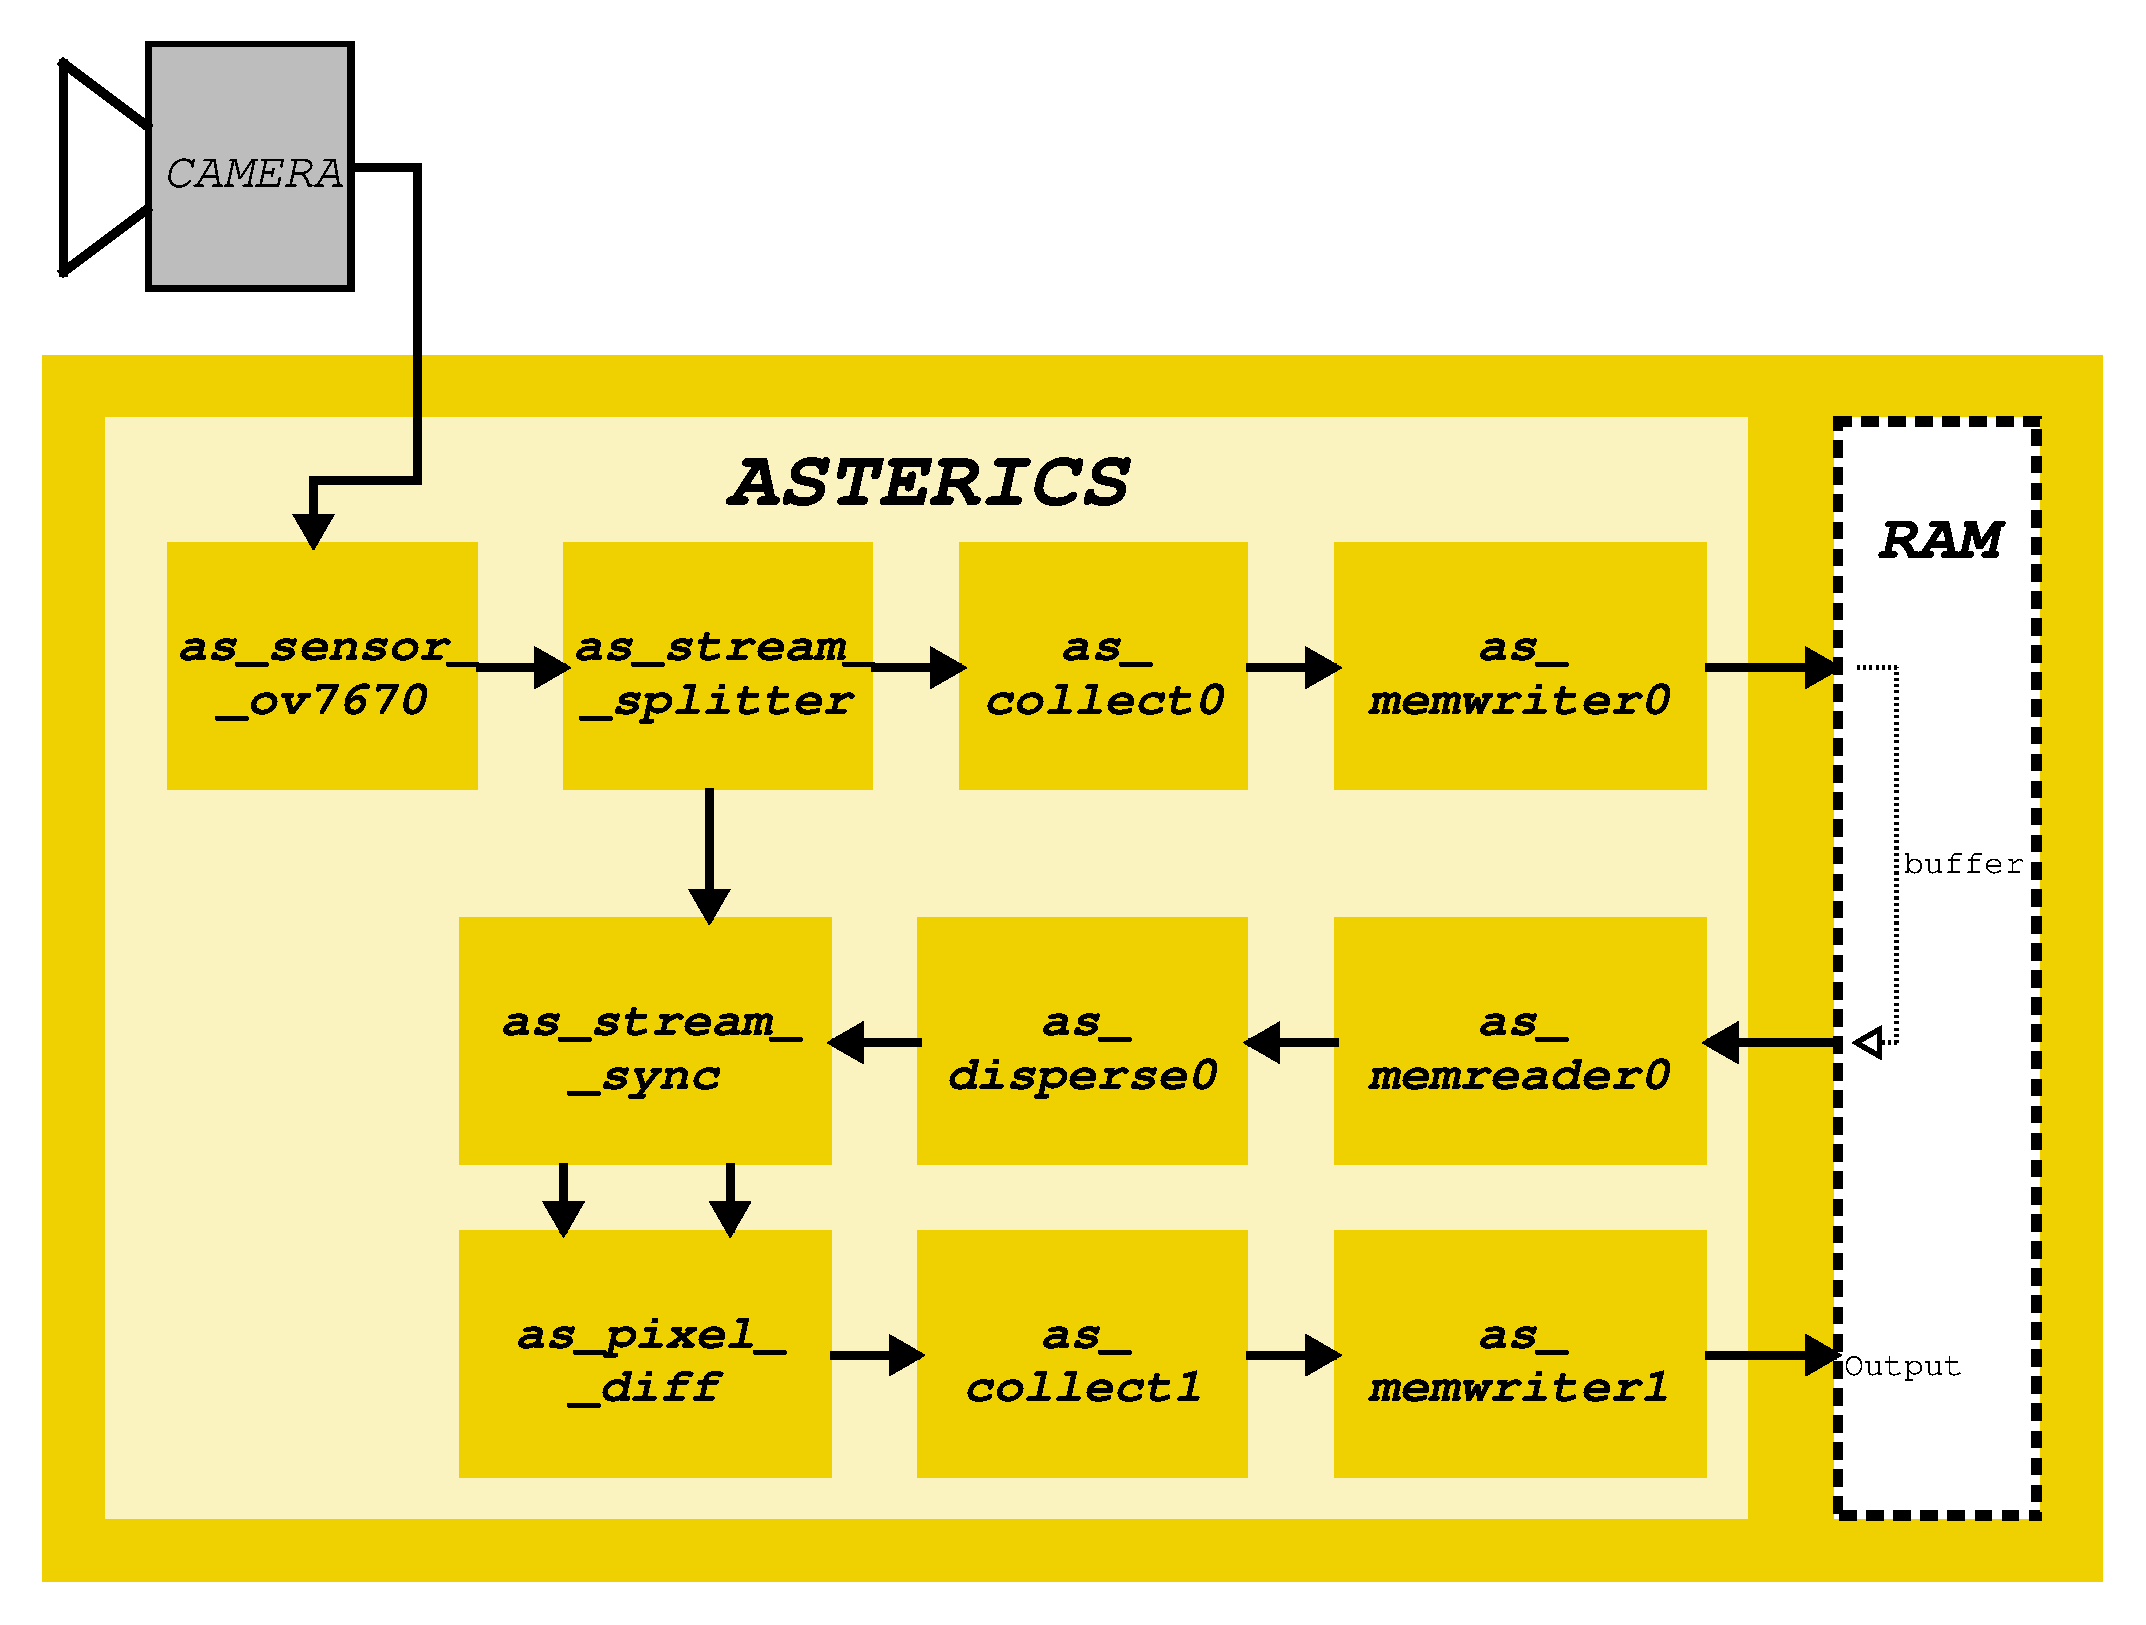
\includegraphics[width=\textwidth]{figs/09-as_refdesign_zybo_image_differencing.pdf}
\caption{Dataflow diagram of the \asterics chain \texttt{as\_refdesign\_zybo}, depicting the included modules.}
\label{fig:09-image_differencing}
\end{figure}

The system architecture is depicted in Figure \ref{fig:09-image_differencing}.
The OV7670 camera is directly connected to the programmable logic and interfaces with an \asterics module \texttt{as\_sensor\_ov7670}.
The physical connection is done via a adapter board or fly-wire connections.
This is detailed in the \texttt{doc} directory of the demo system.
This module converts the camera data stream into a standardized \texttt{as\_stream} interface that the other modules understand.
The data stream is duplicated by the \texttt{as\_stream\_splitter} module.
Each frame is written to RAM by \texttt{as\_memwriter0} from where it is read back when the next frame arrives by the \texttt{as\_memreader0}.
This has the effect of a delay of one frame for this data stream.
The delayed (previous) and duplicated (current) frame are then synchronized by the \texttt{as\_stream\_sync} module and each pixel pair is subtracted from each other by the \texttt{as\_pixel\_diff} module.
The resulting image is then stored in RAM for visualization or further processing.
The \texttt{as\_collect} and \texttt{as\_disperse} modules are used to pack and unpack the eight bit pixel data into 32 bit words for more efficient memory access.
The software for this system is only used to initialize and control the camera and memory access modules and the VEARS core.

This system serves as an example of the capabilities of \asterics and may be used as a starting point and style guide for building your own image processing system using \asterics.
When implemented on the ZyboBoard, switch zero is used to switch between showing the buffered original camera image and the difference image on the screen using the VEARS IP-Core.

For further details regarding building and testing this system, please refer to the included README file and sections \ref{sec:02-getting_started} and \ref{sec:06-02-user_guide}.


\section{as\_refdesign\_canny}
\label{sec:09-01-as_refdesign_canny}
\secauthor{Philip Manke}

\infobox{There are known issues with this system, see section \ref{sec:09-canny_issues}.}

The reference systems \texttt{as\_refdesign\_canny} and \texttt{as\_refdesign\_canny\_dbg} both implement a Canny edge detector using a 2D Window Pipeline subsystem.
Both systems are based on a system developed by Alexander Zoellner and where re-implemented using the 2D Window Pipeline extension of Automatics.
This system is built to demonstrate the 2D Window Pipeline and targets the Zybo-Board development platform.
The system is fully tested for synthesis and implementation using Xilinx Vivado 2019.1.
Note that, just as with the main reference system, \texttt{as\_refdesign\_zybo}, the necessary cable drivers and board files must be installed before building and running the system on hardware.
The system variant \texttt{as\_refdesign\_canny\_dbg} includes additional outputs from the filter modules included in the 2D Window Pipeline, for debugging and educational purposes.

For information on building the system, programming the hardware and operating the software, refer to the README files included in the folders of the systems.

\subsubsection*{System Architecture and Functionality}
\begin{figure}[htbp]
\centering
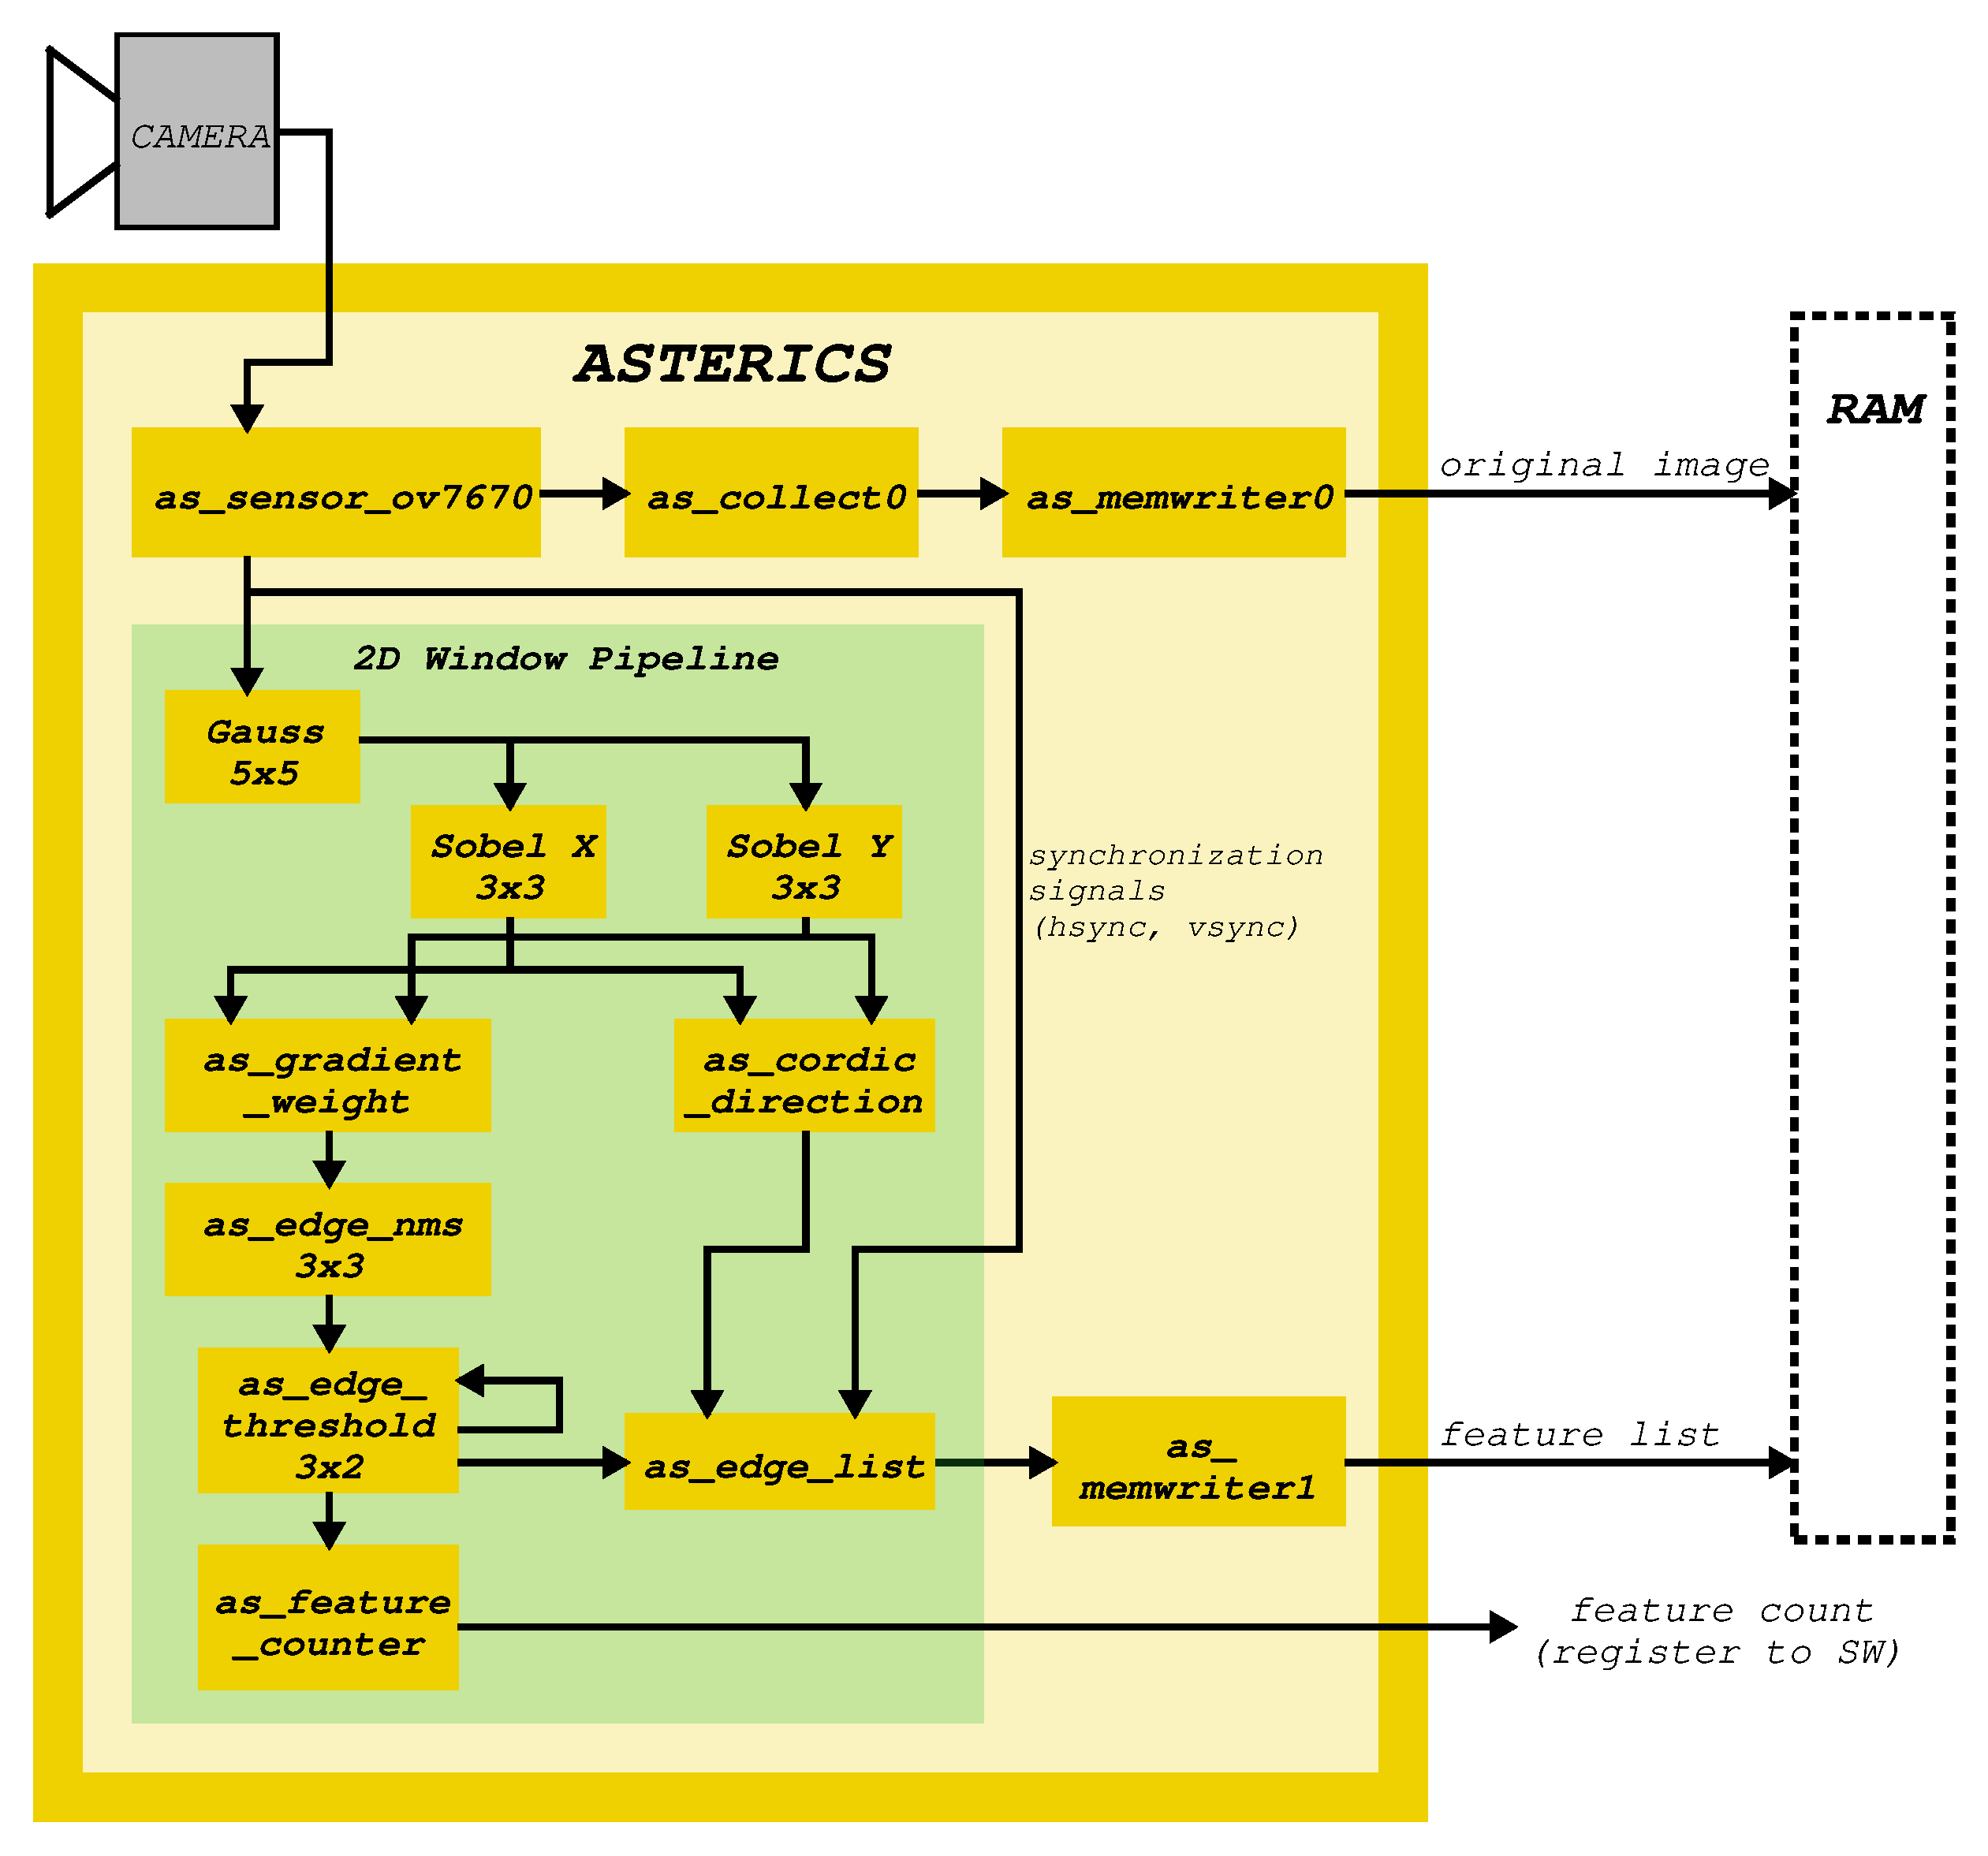
\includegraphics[width=\textwidth]{figs/09-as_refdesign_canny.pdf}
\caption{Dataflow diagram of the \asterics chain \texttt{as\_refdesign\_canny}, depicting the included modules.}
\label{fig:09-canny_diagram}
\end{figure}

The system architecture is depicted in Figure \ref{fig:09-canny_diagram}.
The OV7670 camera is directly connected to the programmable logic and interfaces with the \asterics module \texttt{as\_sensor\_ov7670}.
From there, using the modules \texttt{as\_collect} and \texttt{as\_memwriter}, the original camera image is written to main memory, from where it can be shown on a screen using the VEARS IP-Core, also included with \asterics and in this system.
The Canny edge detector is entirely implemented in a 2D Window Pipeline.
Within the pipeline image convolution with a 5 by 5 Gauss kernel and 3 by 3 Sobel kernels, for both vertical and horizontal edges, is done using three instances of the module \texttt{as\_2d\_conv\_filter\_internal}.
The resulting edge images are combined in the \texttt{as\_gradient\_weight} module and the edge direction is calculated using the Cordic algorithm in the \texttt{as\_cordic\_direction} module.
The combined edge image is filtered for the strongest edge points using a non-maximum-suppression algorithm in the \texttt{as\_edge\_nms} module.
To the now clean edge image, the Canny thresholding is applied in the \texttt{as\_edge\_threshold} module with threshold values provided by software.
The threshold module requires its own output from the last pixel row, requiring a connection to itself.
Lastly this module provides the \texttt{as\_edge\_list} module with the information which pixels are a Canny edge pixel.
The module uses the camera's synchronization signals to generate coordinates for the edge pixels and sends these, together with the Cordic gradient direction to the second \texttt{as\_memwriter} module, writing the Canny features to the main memory.
To inform the software about the number of Canny features written for each camera frame, the \texttt{as\_feature\_counter} module keeps track of the number of Canny edge pixels found and reports that via a slave register.

\section{Known Issues}
\label{sec:09-canny_issues}

This system is not fully tested and debugged.
The following issues unfortunately still exist:

\begin{itemize}
\item The number of reported Canny features per image is not always consistent. In edge cases a very high, incorrect number of features is reported.
\item The memory interface module \texttt{as\_memwriter}, writing the feature data to main memory, sometimes does not finish and reaches a timeout.
\end{itemize}


\section{as\_refdesign\_zynqberry}
\label{sec:09-01-as_refdesign_zynqberry}
\secauthor{Thomas Izycki}

This reference system is designed to serve as a starting point for building processing systems exclusively on the \textit{Zynqberry} using the \asterics framework. The system is tested with Xilinx Vivado 2018.3. Note that just as with all provided reference systems the necessary cable drivers and board files must be installed before building and running the system on hardware.

Beside a \textit{Raspberry Pi} camera v1.3 or 2.1, that has to be connected to the CSI connector, a screen can be attached via HDMI. The system also includes a bare-metal application running on one of the ARM cores, configuring the camera and controlling the ASTERICS chain.

Further information can be obtained by the README files included in the folders of the system.

\subsubsection*{System Architecture and Functionality}

The system architecture is depicted in Figure \ref{fig:09-zynqberry-video-stream}.

\begin{figure}[htbp]
    \centering
    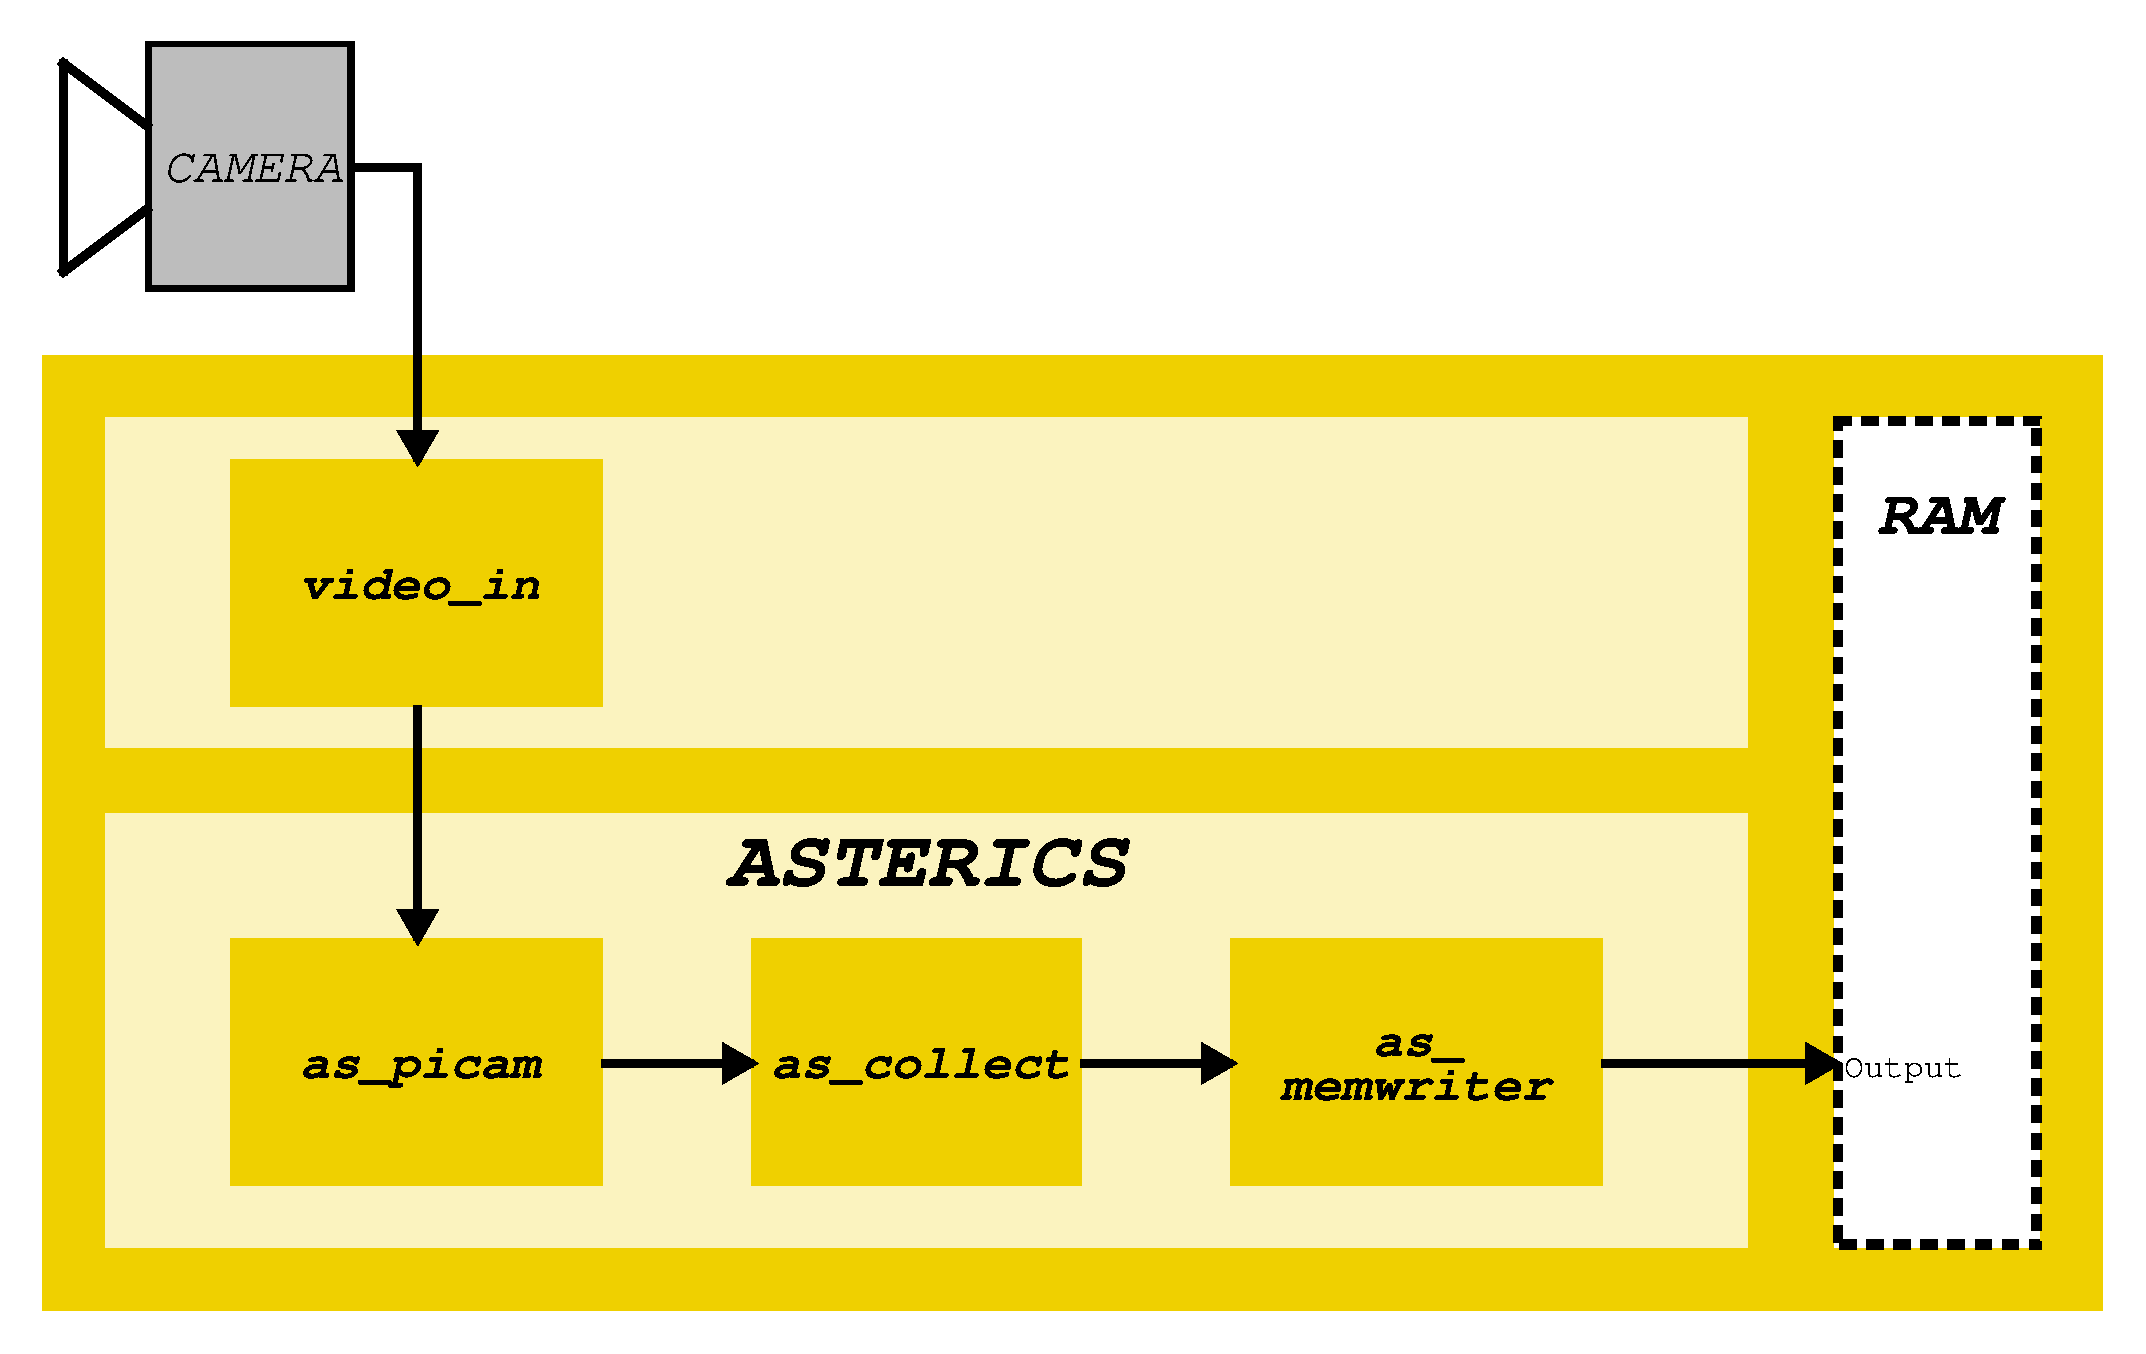
\includegraphics[width=\textwidth]{figs/09-as_refdesign_zynqberry.pdf}
    \caption{Dataflow diagram of the \asterics chain \texttt{as\_refdesign\_zynqberry}, depicting the included modules.}
    \label{fig:09-zynqberry-video-stream}
\end{figure}

 A \textit{Raspberry Pi} camera v1.3 or v2.1 is connected to the \texttt{video\_in} submodule that is not part of the \asterics framework but provided by \textit{Trenz Electronic GmbH} and included in this reference system. The following \texttt{as\_picam} module converts the data stream into a standardized \texttt{as\_stream} interface and computes the grayscale values of the camera images. Subsequent to this module, an own \asterics image processing chain can be built up. In the present case no further image processing takes place and the \texttt{as\_collect} module is used to pack the 8-bit pixel data into 32-bit words for more efficient memory access. The \texttt{as\_memwriter} module writes the images to the main memory. Using the \asterics module for visualization (\textit{VEARS}) IP-Core, the images are shown on the screen attached to the HDMI connector.

 While connected to a computer, the standard output can be displayed on a serial console and might be useful to check the status of the system on start up.
